\documentclass[tikz]{standalone}
\begin{document}
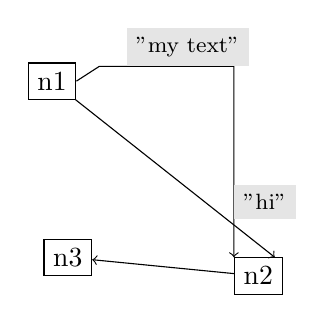
\begin{tikzpicture}[n/.style={rectangle,draw,align=center},e/.style={draw,->},t/.style={rectangle,draw=none,fill=black!10,align=center,font=\footnotesize}]

\node[n] (n1) at (2mm, -3mm) {n1};
\node[n, anchor=north west] (n2) at ([xshift=+20mm, yshift=-20mm] n1.south east) {n2};
\node[n, anchor=center] (n3) at ([xshift=2mm] n1 |- n2.north) {n3};
\path[e] (n2) -- (n3);
\path[e] (n1.east) -- (8mm, -3.2pt) -| (n2.north west) node[t, anchor=south west, pos=0.1](myLabel) {"my text"} node[t, anchor=south west, pos=0.9] {"hi"};
\path[e] (n1) -- ([xshift=-1mm] n2.north east);

\end{tikzpicture}
\end{document}
